
%%%% OK

In this section we discuss the context underlining our contribution and present the motivations that led to our approach.

\subsection{Context: Mobile Crowd-Sensing Platforms}

The crowd-sensing platforms have a large application domain.
The applications encompass application performance monitoring (\emph{e.g.}, OpenSignal\footnote{\url{http://opensignal.com}}), environment monitoring (air quality\footnote{\url{http://citizensensor.cc}}), etc.
\\

Privacy-preserving in this context is a key challenge to address.
The platforms must balance to find an equilibrium between the level of the users' privacy-preserving and the quality of the data that are collected.
Indeed, if a crowd-sensing platform put a lot of consideration in the privacy preserving, the collected data could be degraded depending to the data type.
At last, if a crowd-sensing platform does not care about the privacy of its users, the latter may not want to contribute to it.
To the best of our knowledge, privacy-preserving techniques are often deployed on the server side~\cite{DBLP:conf/mobisys/CorneliusKKPST08}~\cite{DBLP:conf/dais/HadererRS13}.
For instance, for the Geo-located data, there can be anonymized \emph{a posteriori}~\cite{DBLP:conf/icdcs/PrimaultMB15}.
\\

The context to this proposal is based on the APISENSE crowd-sensing platform that provide an Android application to collect data from users.
Those users subscribe to data collect campaign and contribute with their mobile devices.
Because the platform applies privacy-preserving techniques on the server side, it does not protect from malicious behaviors during the upload phase.
The data coming from a user are unmodified and are his own data.
Those data were produced by this specific user.
A user is, therefore, forced to trust the server that receives his data.

\subsection{Motivations: Data Dissemination Threats}

In the APISENSE platform, a collect server, also called Honeycomb, can be managed by an external organization.
\\

Having multiple servers is a requirement because a single server cannot handle all users' data that are sent during a collect campaign.
Moreover, for the users' privacy, no server can be trusted.
\\

A key challenge in the crowd-sensing platforms is to avoid central trusted server that present a single point of failure that need to be addressed.

\begin{figure*}[h]
    \centering
    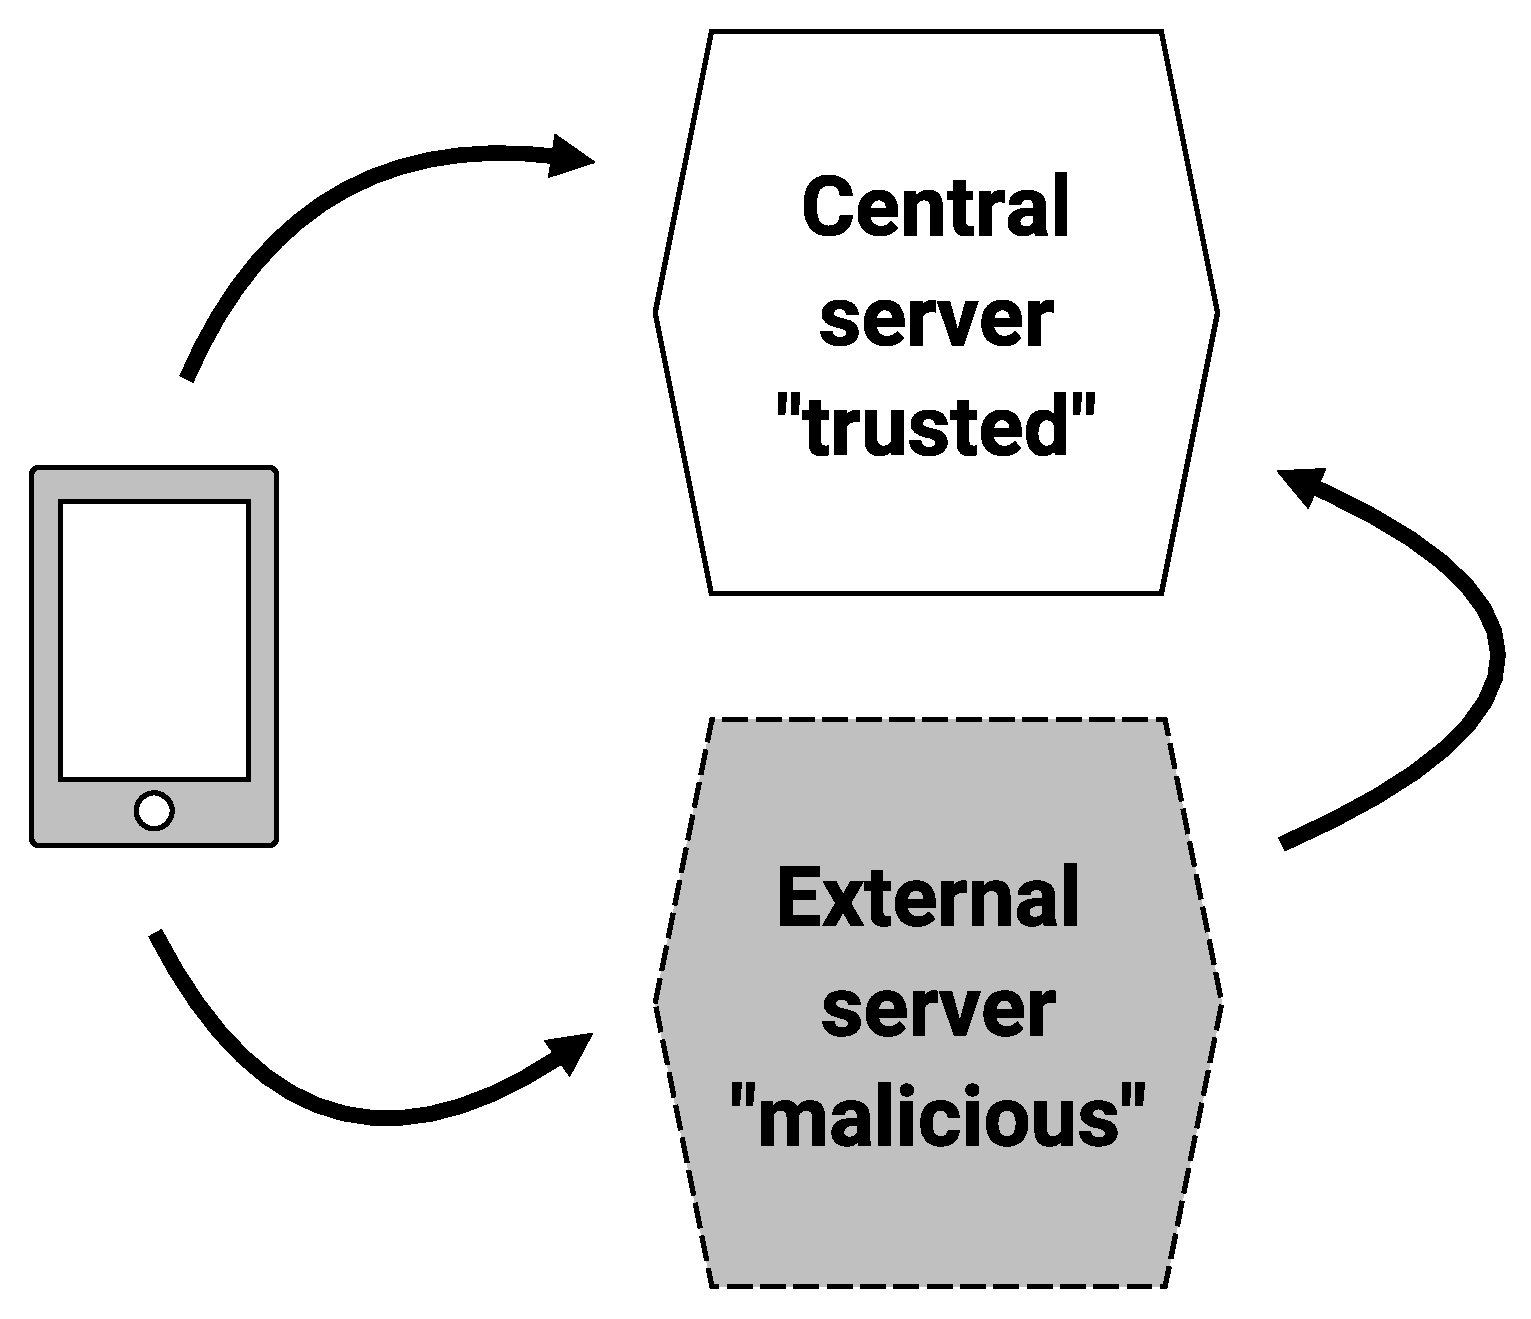
\includegraphics[width=0.5\textwidth]{figures/threat}
    \caption{\label{Threat} APISENSE data collection threat}
\end{figure*}

The current process of data collection is represented in Figure~\ref{Threat}.
\\

Let assume a user that participates to a data collect campaign.
Currently, the user produces data and sends it directly to a collect server.
The user has no control on the server selection that will receive the data.
The server that receives the data knows irremediably that those data are produced by the user that sends it.
The server that collects the data can be a trusted server or, as exposed before, an external server managed by an organization that can be potentially malicious.
The threat on a malicious server is that it can use the data against the user and deduct privacy information about it.
Furthermore, even if the data are collected by a trusted collect server, the threat can come from a malicious person that listen the transmission channels or steals the data stored on the server.
This kind of threats is not viable for privacy concerns.
\\

To address these threat scenarios, we think of a method where a user is able to send data that he does not produce: data that come from other users.
With this decentralized approach, the data associated to a user on the server can be produced by any other else user on the system.
Even if the data are leaked, the privacy of a user is not compromised.

\subsection{Goal: Enabling Decentralized Dissemination}

The main goal is to provide a decentralized data dissemination approach that could protect the users' privacy in an untrusted environment.
We want to tend to a solution that could take the advantages of a Privacy by design approach which leads to a minimal intrinsically privacy-preserving system.
Ultimately, our objective is to break the ability of an end-server to link a data to his producer without compromising the quality and the utility of the whole dataset.

%%%% END OK
